\batchmode
\documentclass[a4paper,10pt]{article}
\usepackage{graphicx}
\usepackage{fancyvrb}
\usepackage{color}
\usepackage{xcolor}
\usepackage{verbatim}
\usepackage{amssymb}
\usepackage{amsmath}
\usepackage{hyperref}
\usepackage{natbib}
\usepackage{caption}
\usepackage{subcaption}
\usepackage{nameref}

\hypersetup{urlcolor=blue, colorlinks=true} 
\usepackage{float}

%used in SL section
\usepackage{mathptmx}
\usepackage{siunitx} %SI-einheiten
\usepackage{lmodern} %weitere mathematischen Symbole
\usepackage{placeins} %floatbarrier

\DeclareSIUnit\parsec{pc}
\DeclareSIUnit\lightyear{ly}
\DeclareSIUnit\year{yr}
\DeclareSIUnit\erg{erg}
\DeclareSIUnit\ster{ster}
\DeclareSIUnit\arcsec{arcsec}
\DeclareSIUnit\deg{deg}

\definecolor{gruen}{cmyk}{0.35,0.01,0.80,0.1}

\textheight=25.5cm
\textwidth=17.5cm
\voffset=0.cm
\hoffset=-0.0cm
\oddsidemargin -1cm
\evensidemargin -1cm
\topmargin -2cm
\baselineskip=0.900cm
\setlength{\parindent}{0in}

\graphicspath{{../figures/}}

\providecommand{\e}[1]{\ensuremath{\times 10^{#1}}}
\newcommand{\given}[2]{\ensuremath{P(#1|#2)}}
\newcommand{\x}[0]{\ensuremath{\vec{x}}}
\newcommand{\gauss}[3]{\ensuremath{\frac{1}{\sqrt{2\pi#2^2}}\text{exp}\left(- \frac{(#1-#3)^2}{2#2^2}\right)}}

\newcommand{\ttt}[1]{\texttt{#1}}
\newcommand{\clB}[1]{\textcolor{blue}{#1}}

% used in SL section
\newcommand{\todo}[2]{\textcolor{red}{\textbf{TODO (#1): #2}}}

\title{LSS: Summary}
\author{Humna Awan, Eric Gawiser}
\date{\today}

\begin{document}
\maketitle
%%%%%%%%%%%%%%%%%%%%%%%%%%%%%%%%%%%%%%%%%%%%%%%%%%%%%%%%%%%
\section*{Summary}
Our list of metrics include:
\enumerate{
\item \nameref{median visits}
\item \nameref{rotational dithers}
\item \nameref{translational dithers}
\item \nameref{area}
\item \nameref{median depth}
\item \nameref{depth std}
\item \nameref{OS systematics}
\item \nameref{4MOST+DESI overlap}
\item \nameref{seeing}
}\

\noindent\clB{I can finish the description of the interactions of these metrics later today.}

%%%%%%%%%%%%%%%%%%%%%%%%%%%%%%%%%%%%%%%%%%%%%%%%%%%%%%%%%%%
\newpage
\section*{Median Number of Visits Per Field (After Y10)\label{median visits}}
This metric ensures that we are meeting the LSST SRD requirement that the median number of WFD visits per field after Y10 is at least 825.

\begin{minipage}{\columnwidth}
\centering
 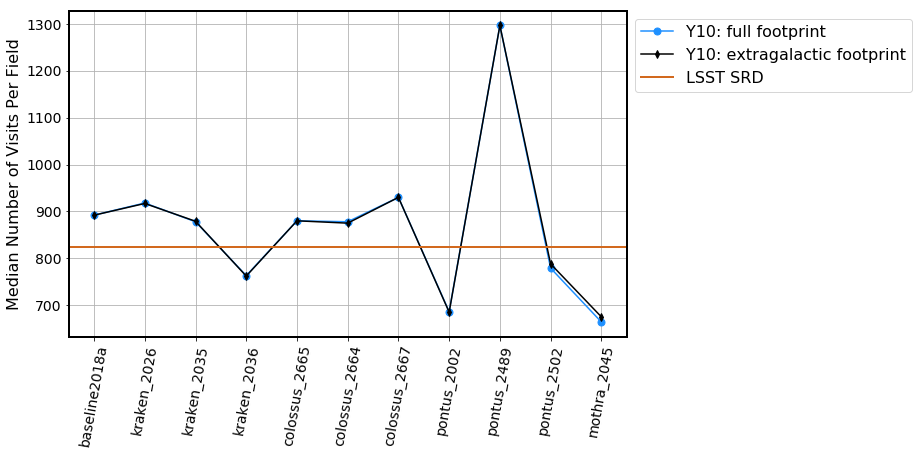
\includegraphics[width=.9\columnwidth]{lss_compare_median_nvisits_11dbs.png}
\end{minipage}

\clB{Will add the rest of the cadences (especially \ttt{alt\_sched} and \ttt{FBS} outputs) but need to create a \ttt{Stacker} for \ttt{fieldIDs} since the new schedulers don't have \ttt{fieldIDs} associated with visits.}

%%%%%%%%%%%%%%%%%%%%%%%%%%%%%%%%%%%%%%%%%%%%%%%%%%%%%%%%%%%
\newpage
\section*{Rotational Uniformity\label{rotational dithers}}
This metric looks at the distributions of \ttt{rotTelPos} and \ttt{rotSkyPos} as we'd like them to be uniform. The nominal pointings leads a pile-up in \ttt{rotTelPos} distribution at +/-90, 0 degrees. We see that rotational dithers help achieve more uniform distributions (and we understand the pile-up at 0 deg in the dithered \ttt{rotTelPos} distribution: there are visits that do not get dithered under the current rotational dithering scheme).

\begin{minipage}{\columnwidth}
\centering
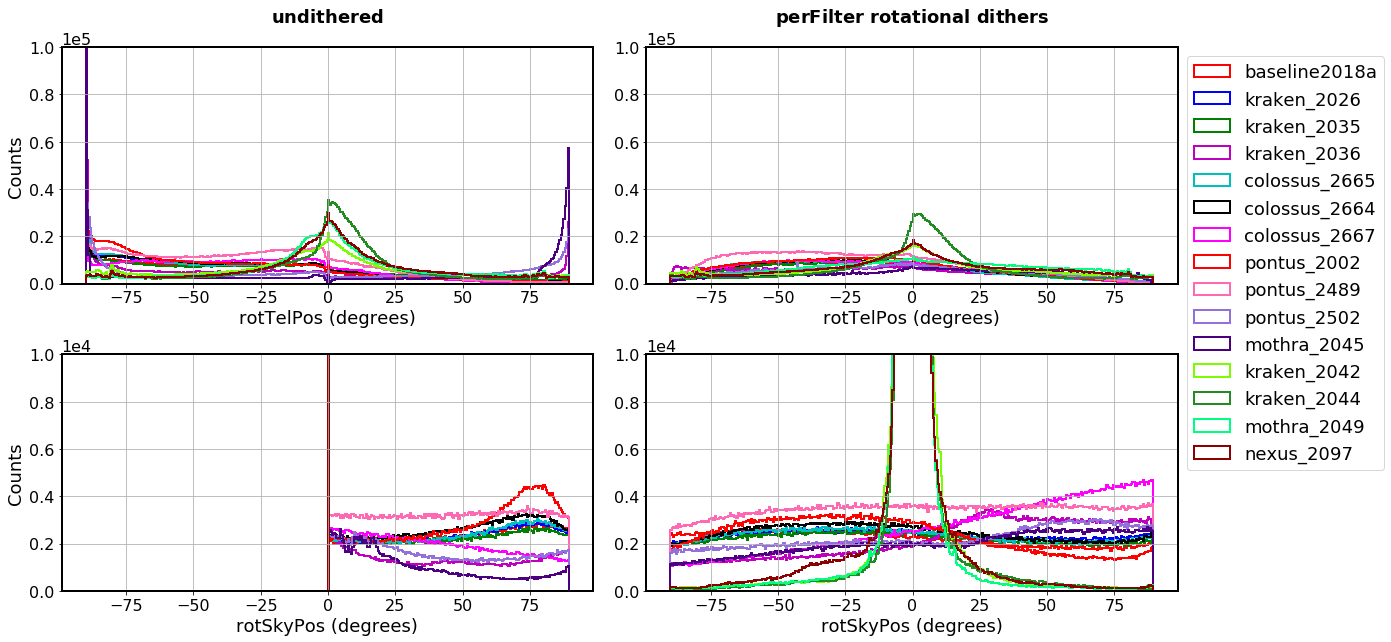
\includegraphics[width=\columnwidth]{lss_compare_rotDiths_15dbs.png}
\end{minipage}

\clB{The right column will be updated once we have per night rotational dithers. Hopefully it'll fix the pile-up at zero in the dithered \ttt{rotTelPos} distribution (and consequently the \ttt{rotSkyPos} distribution). Also, the outputs from new schedulers need to be added.}

%%%%%%%%%%%%%%%%%%%%%%%%%%%%%%%%%%%%%%%%%%%%%%%%%%%%%%%%%%%
\newpage
\section*{Translational Uniformity\label{translational dithers}}
This metric looks at the need for (large) translational dithers. An undithered survey not only leads to survey non-uniformity but also a comparatively shallower survey. We showed in Awan+16 that translational dithers help with both issues.

\begin{minipage}{\columnwidth}
\centering
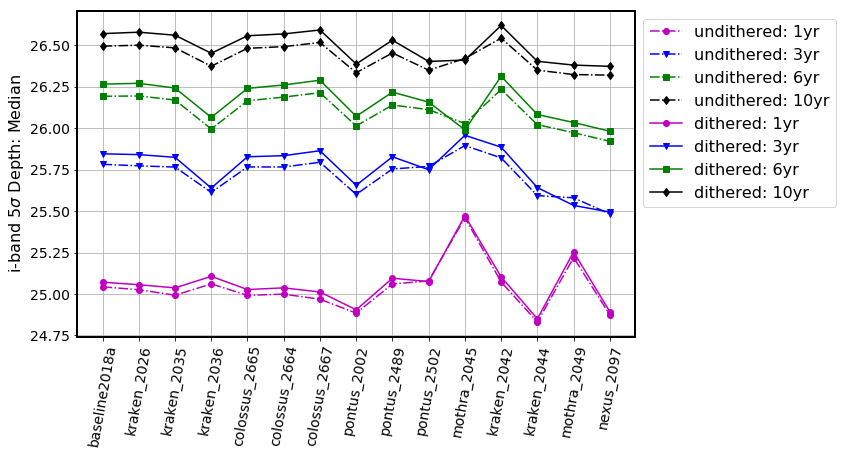
\includegraphics[width=.75\columnwidth]{lss_compare_depth_median_15dbs_undith.png}
\end{minipage}

Here, the dithered survey implemented per night, random translational dithers, as large as the LSST FOV. Also, the median depth is for the extragalactic footprint.

%%%%%%%%%%%%%%%%%%%%%%%%%%%%%%%%%%%%%%%%%%%%%%%%%%%%%%%%%%%
\newpage
\section*{Extragalactic Footprint\label{area}}
This metric looks at the usable area for extragalactic science, which we achieve by implementing an extinction cuts and a depth cut on the coadded depth footprint.  Specifically, we retain only the area with E(B-V) $<$ 0.2 with limiting $i$-band coadded 5$\sigma$ depth of 24.5 for Y1, 25.0 for Y3, 25.5 for Y6, and 26.0 for Y10.

\begin{minipage}{\columnwidth}
\centering
 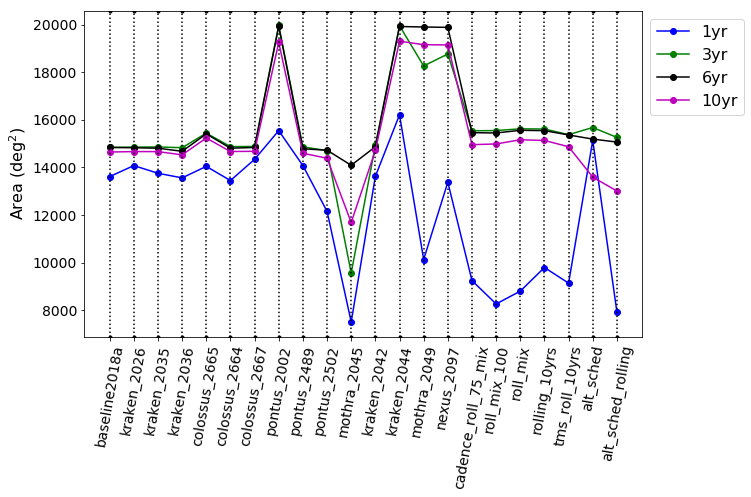
\includegraphics[width=.75\columnwidth]{lss_compare_area_22dbs.png}
\end{minipage}

\clB{This figure will be updated once we cater our depth cuts to each cadence}.

%%%%%%%%%%%%%%%%%%%%%%%%%%%%%%%%%%%%%%%%%%%%%%%%%%%%%%%%%%%
\newpage
\section*{Median Depth in the Extragalactic Footprint\label{median depth}}
This metric looks at the median depth in the extragalactic footprint. We would like to go deeper to probe a fainter galaxy sample to get better constraining power. Here, we look at the $i$-band coadded 5$\sigma$ depth after Y1, 3, 6, 10.

\begin{minipage}{\columnwidth}
\centering
 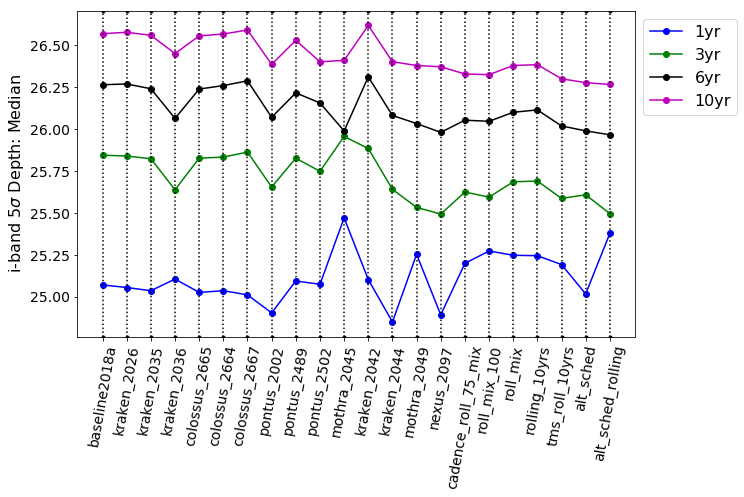
\includegraphics[width=.75\columnwidth]{lss_compare_depth_median_22dbs.png}
\end{minipage}

\clB{This figure will be updated once we cater our depth cuts to each cadence}.

%%%%%%%%%%%%%%%%%%%%%%%%%%%%%%%%%%%%%%%%%%%%%%%%%%%%%%%%%%%
\newpage
\section*{Depth Uniformity in the Extragalactic Footprint\label{depth std}}
This metric looks at the depth uniformity in the extragalactic footprint. Here, we model this as the standard deviation in the $i$-band coadded 5$\sigma$ depth in the extragalactic footprint.  We would like to minimize non-uniformity to minimize window function uncertainties. 

\begin{minipage}{\columnwidth}
\centering
 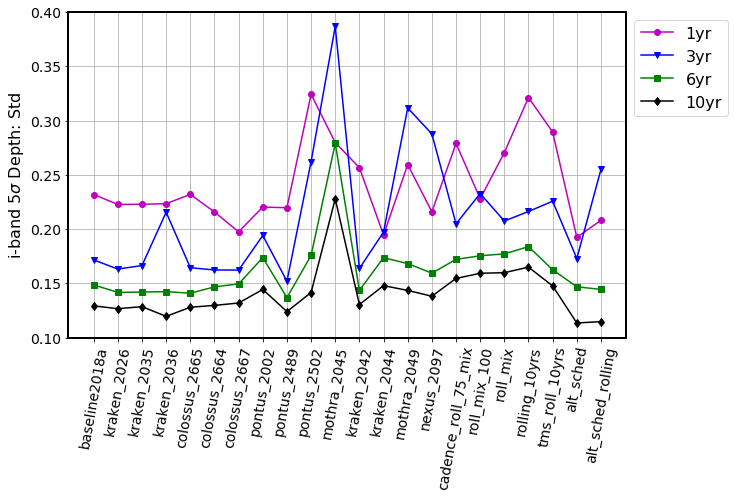
\includegraphics[width=.75\columnwidth]{lss_compare_depth_std_22dbs.png}
\end{minipage}

\clB{This figure will be updated once we cater our depth cuts to each cadence}.

%%%%%%%%%%%%%%%%%%%%%%%%%%%%%%%%%%%%%%%%%%%%%%%%%%%%%%%%%%%
\newpage 
\section*{Impacts of Artificial Structure\label{OS systematics}}
This metric looks at the effectiveness of each cadence in minimizing the uncertainties in the artificial structure that is induced the observing strategy. It is an implementation of Equation 9.4 in LSST Observing Strategy Community White Paper.

\clB{This figure should be ready by 10/21/18}.

\begin{minipage}{\columnwidth}
\centering
% 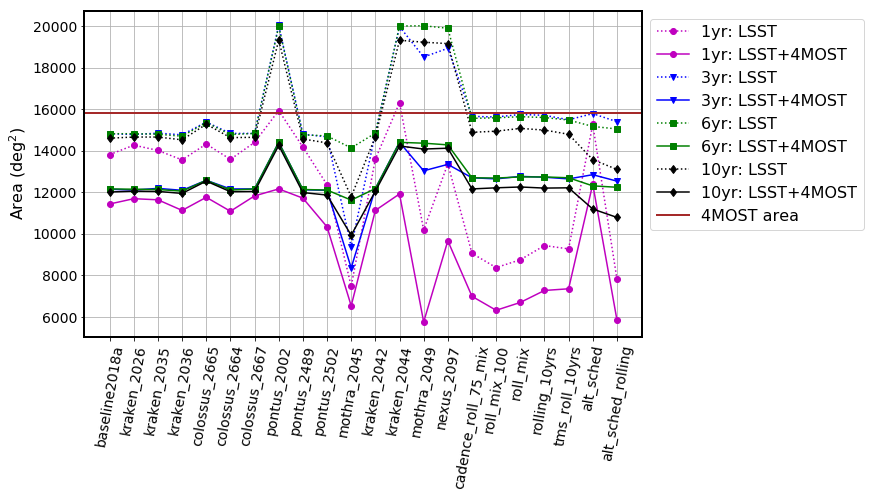
\includegraphics[width=.75\columnwidth]{lss_compare_4MOSToverlap_22dbs.png}
\end{minipage}

%%%%%%%%%%%%%%%%%%%%%%%%%%%%%%%%%%%%%%%%%%%%%%%%%%%%%%%%%%%
\newpage
\section*{4MOST(+DESI) Overlap\label{4MOST+DESI overlap}}
This metric looks at the overlap between LSST footprint and spectroscopic surveys like 4MOST and DESI.

\begin{minipage}{\columnwidth}
\centering
 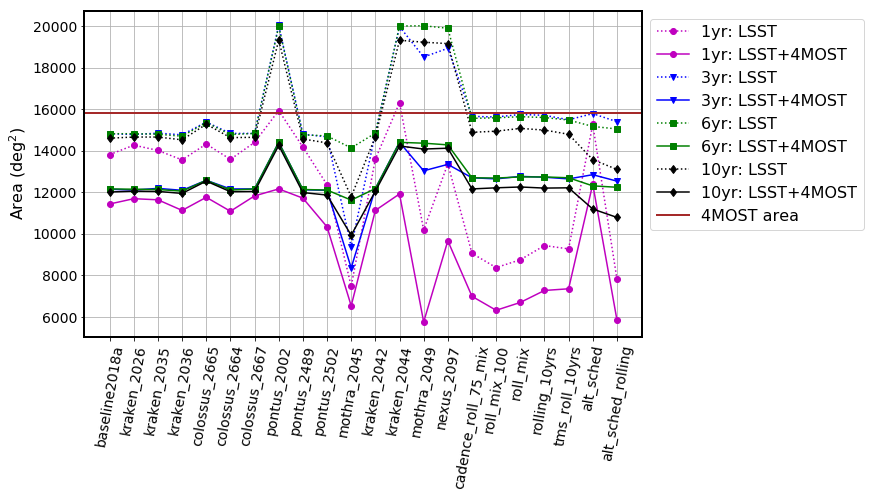
\includegraphics[width=.8\columnwidth]{lss_compare_4MOSToverlap_22dbs.png}
\end{minipage}

\clB{This figure will be updated since I received the DESI footprint a short while ago. We would like the footprint with either 4MOST or DESI overlap (not necessarily both). Also, we need to quantify the minimum size of spectroscopic sample needed for our photo-z calibrations}.

%%%%%%%%%%%%%%%%%%%%%%%%%%%%%%%%%%%%%%%%%%%%%%%%%%%%%%%%%%%
\newpage
\section*{Impacts of Seeing\label{seeing}}
This metric looks at the impacts of seasonal variations in seeing, as implemented by Eric Nielson. It is critical to get a more realistic seeing implemented in our simulated cadences as ignoring seeing variations leads to inaccurate calculation of the 5$\sigma$ point-source depth which impacts all derived quantities, e.g. the coadded 5$\sigma$ depth.

\begin{minipage}{\columnwidth}
\centering
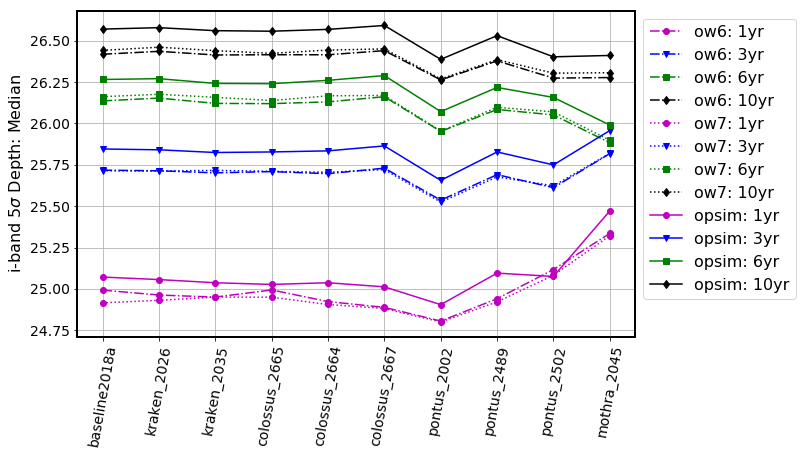
\includegraphics[width=.75\columnwidth]{lss_compare_depth_median_10dbs_ow6_ow7_opsim.png}
\end{minipage}

Here, \ttt{ow6} and \ttt{ow7} identify two different outputs from \ttt{owsee}, using data from different but overlapping years in Pachon.


\end{document}
